\documentclass[10pt]{beamer}
\usetheme{metropolis}
\usepackage[utf8]{inputenc}
\usepackage{booktabs}
\usepackage{graphicx}
\usepackage{amsmath}
\usepackage{amssymb}
\usepackage{tikz}

\title{The Janus Rotational System}
\subtitle{Dynamic Market Regime Detection \& Momentum Smoothing}
\date{\today}
\author{Tactical Alpha Research}
\institute{Academic Portfolio Management Suite}

\begin{document}

\maketitle

\begin{frame}{Institutional Glossary \& Definitions}
    \begin{itemize}
        \item \textbf{CAGR}: Compound Annual Growth Rate (Geometric mean return).
        \item \textbf{Sharpe Ratio}: Risk-adjusted return (Excess Return / Volatility).
        \item \textbf{SMA (200)}: 200-day Simple Moving Average (Primary Trend filter).
        \item \textbf{MACD Confirmation}: Moving Average Convergence Divergence used to filter whipsaws.
        \item \textbf{Tranche Laddering}: Staggered trade execution over $N$ weeks.
        \item \textbf{60/40 Benchmark}: A portfolio of 60\% Global Equities and 40\% Bonds.
    \end{itemize}
\end{frame}

% ── Section 1: Philosophy & Foundation ───────────────────────────────────
\section{Philosophy \& Strategy Architecture}

\begin{frame}{Abstract: The Multi-Asset Challenge}
    \textbf{Target}: Outperform the 60/40 benchmark on a risk-adjusted basis through tactical de-risking.
    \vspace{0.3cm}
    \begin{itemize}
        \item \textbf{The Problem}: Standard 60/40 portfolios suffer significant "Bond-Drain" during synchronized correlations (e.g., 2022).
        \item \textbf{The Goal}: A system that transitions from 100\% Equity concentration to 100\% Safe-Haven protection via structural catalysts.
        \item \textbf{Key Insight}: Performance persistence is found at the intersection of \textit{Fundamental Health} and \textit{Trend Discipline}.
    \end{itemize}
\end{frame}

\begin{frame}{Janus System Architecture}
    \begin{center}
    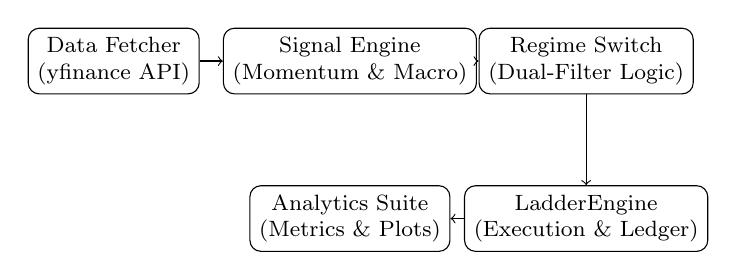
\begin{tikzpicture}[node distance=1.5cm, every node/.style={draw, rectangle, font=\footnotesize, align=center, rounded corners}]
        \node (data) {Data Fetcher\\(yfinance API)};
        \node (signal) [right of=data, xshift=1.5cm] {Signal Engine\\(Momentum \& Macro)};
        \node (regime) [right of=signal, xshift=1.5cm] {Regime Switch\\(Dual-Filter Logic)};
        \node (engine) [below of=regime, yshift=-0.5cm] {LadderEngine\\(Execution \& Ledger)};
        \node (report) [left of=engine, xshift=-1.5cm] {Analytics Suite\\(Metrics \& Plots)};
        
        \draw[->] (data) -- (signal);
        \draw[->] (signal) -- (regime);
        \draw[->] (regime) -- (engine);
        \draw[->] (engine) -- (report);
    \end{tikzpicture}
    \end{center}
    \begin{itemize}
        \item \textbf{Modularity}: Decoupled components allow for independent stress-testing of each alpha source.
        \item \textbf{Integrity}: Vectorized execution engine ensures zero look-ahead bias and backtest fidelity.
    \end{itemize}
\end{frame}

\begin{frame}{Core Logic: The Double-Filter Engine}
    \textbf{The Logic of Conservatism}:
    The system defines a \textbf{Bull State} only if \textit{Both} filters are satisfied. If \textit{Either} fails, the system triggers systematic de-risking. This is a "Fail-Safe" for capital preservation.
    \vspace{0.4cm}
    \begin{itemize}
        \item \textbf{Fundamental Filter}: Structural Earnings / ROE health of US Mega-Caps.
        \item \textbf{Technical Filter}: Trend Confirmation via 200-SMA \& MACD (12/26).
    \end{itemize}
    \vspace{0.3cm}
    \[ \text{Regime} = [\text{Fund} > \theta] \wedge [\text{P} > \text{SMA}_{200} \wedge \text{MACD} > 0] \]
\end{frame}

\begin{frame}{The Fundamental Filter: Rationale}
    \begin{itemize}
        \item \textbf{Variable}: Composite ROE and Earnings Stability of the SPY Top-10.
        \item \textbf{Lag Constraint}: All data is lagged by \textbf{45 calendar days} to account for reporting cycles.
        \item \textbf{Logic}: Deterioration beyond 2-sigma thresholds marks a structural macro regime shift.
    \end{itemize}
\end{frame}

\begin{frame}{The Technical Filter: Path Persistence}
    Macro indicators are slow; technicals provide the "path" confirmation.
    \begin{itemize}
        \item \textbf{Criterion A}: Price above 200-day Simple Moving Average (SMA).
        \item \textbf{Criterion B}: MACD Histogram (12/26) must be $> 0$.
    \end{itemize}
    \textbf{Why both?}: SMA establishes the primary trend; MACD confirms the internal momentum to avoid false turn-arounds in shallow dips.
\end{frame}

\begin{frame}{Visualizing the Regime (Figure 1)}
    \begin{center}
        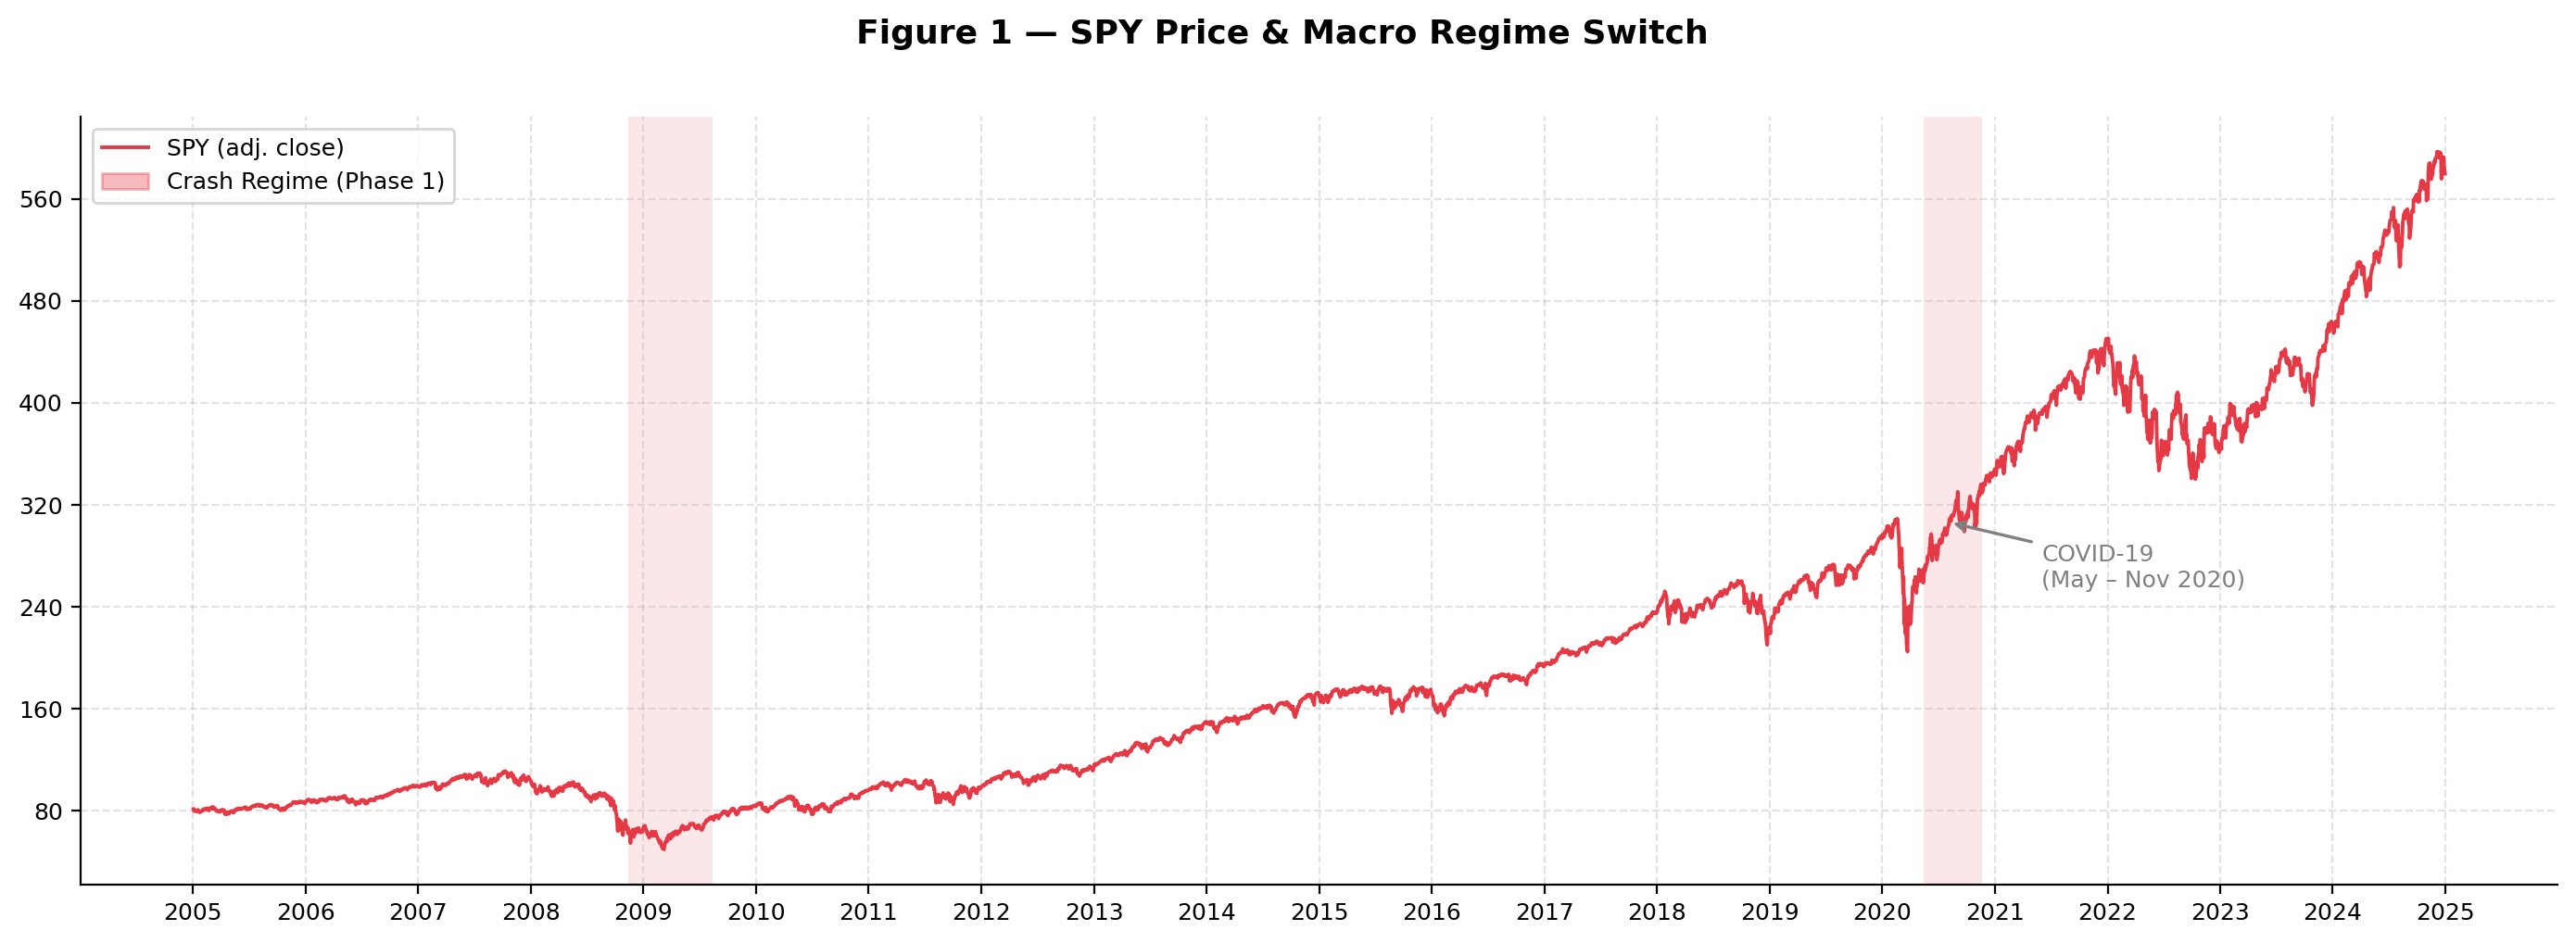
\includegraphics[width=\textwidth,height=0.7\textheight,keepaspectratio]{../plots/figure_1_regime_overlay.png}
    \end{center}
    \textbf{Standalone Insight}:
    \footnotesize Every red band represents a systematic exit from the SPY into Safe-Haven bonds/cash. The 2008 exit occurred \textit{before} the 50\% drawdown peak, preserving significant principal.
\end{frame}

% ── Section 2: Tactical Selection ────────────────────────────────────────
\section{Active Selection \& Execution Mechanics}

\begin{frame}{Dual Momentum Selection}
    \textbf{Rationale}: Relative strength ranking ensures we only hold the "Winningest" assets in any regime.
    \vspace{0.4cm}
    \[ RS_i = \omega_1 R_{i, 63d} + \omega_2 R_{i, 126d} \]
    \vspace{0.3cm}
    \begin{itemize}
        \item \textbf{Tactical (63d)}: 3-month momentum captures sector rotations and earnings cycles.
        \item \textbf{Structural (126d)}: 6-month momentum ensures we are aligned with long-term money flows.
        \item \textbf{Output}: Top-5 assets daily (Equal-Weighted).
    \end{itemize}
\end{frame}

\begin{frame}{Universe Segregation Logic}
    Strategic separation prevents "Bond-Drain" in growth regimes:
    \vspace{0.3cm}
    \begin{itemize}
        \item \textbf{Equity Universe}: 30 Diversified Sector \& Global ETFs (SPY, QQQ, XLK, MGK, etc.).
        \item \textbf{Safe-Haven Universe}: 10 Low-Correlated Bond/Cash ETFs (BNDX, TLT, TIP, BIL).
    \end{itemize}
    \vspace{0.3cm}
    \textbf{Policy}: In Bull regimes, bond allocation is zeroed. In Bear regimes, equity is zeroed.
\end{frame}

\begin{frame}{The Execution Ledger: LadderEngine}
    \textbf{Problem}: Standard backtests ignore "Timing Risk"—the risk of rebalancing on a uniquely good/bad day.
    \vspace{0.3cm}
    \begin{itemize}
        \item \textbf{The Solution}: 4-Tranche Sequential Deployment.
        \item \textbf{Process}: Tranche $T_1$ rebalances Week 1, $T_2$ Week 2, etc.
        \item \textbf{Effect}: Atomizes the portfolio into four distinct sub-backtests that are averaged at the portfolio level, significantly smoothing returns.
    \end{itemize}
\end{frame}

\begin{frame}{Dynamic Capital Allocation (Figure 2)}
    \begin{center}
        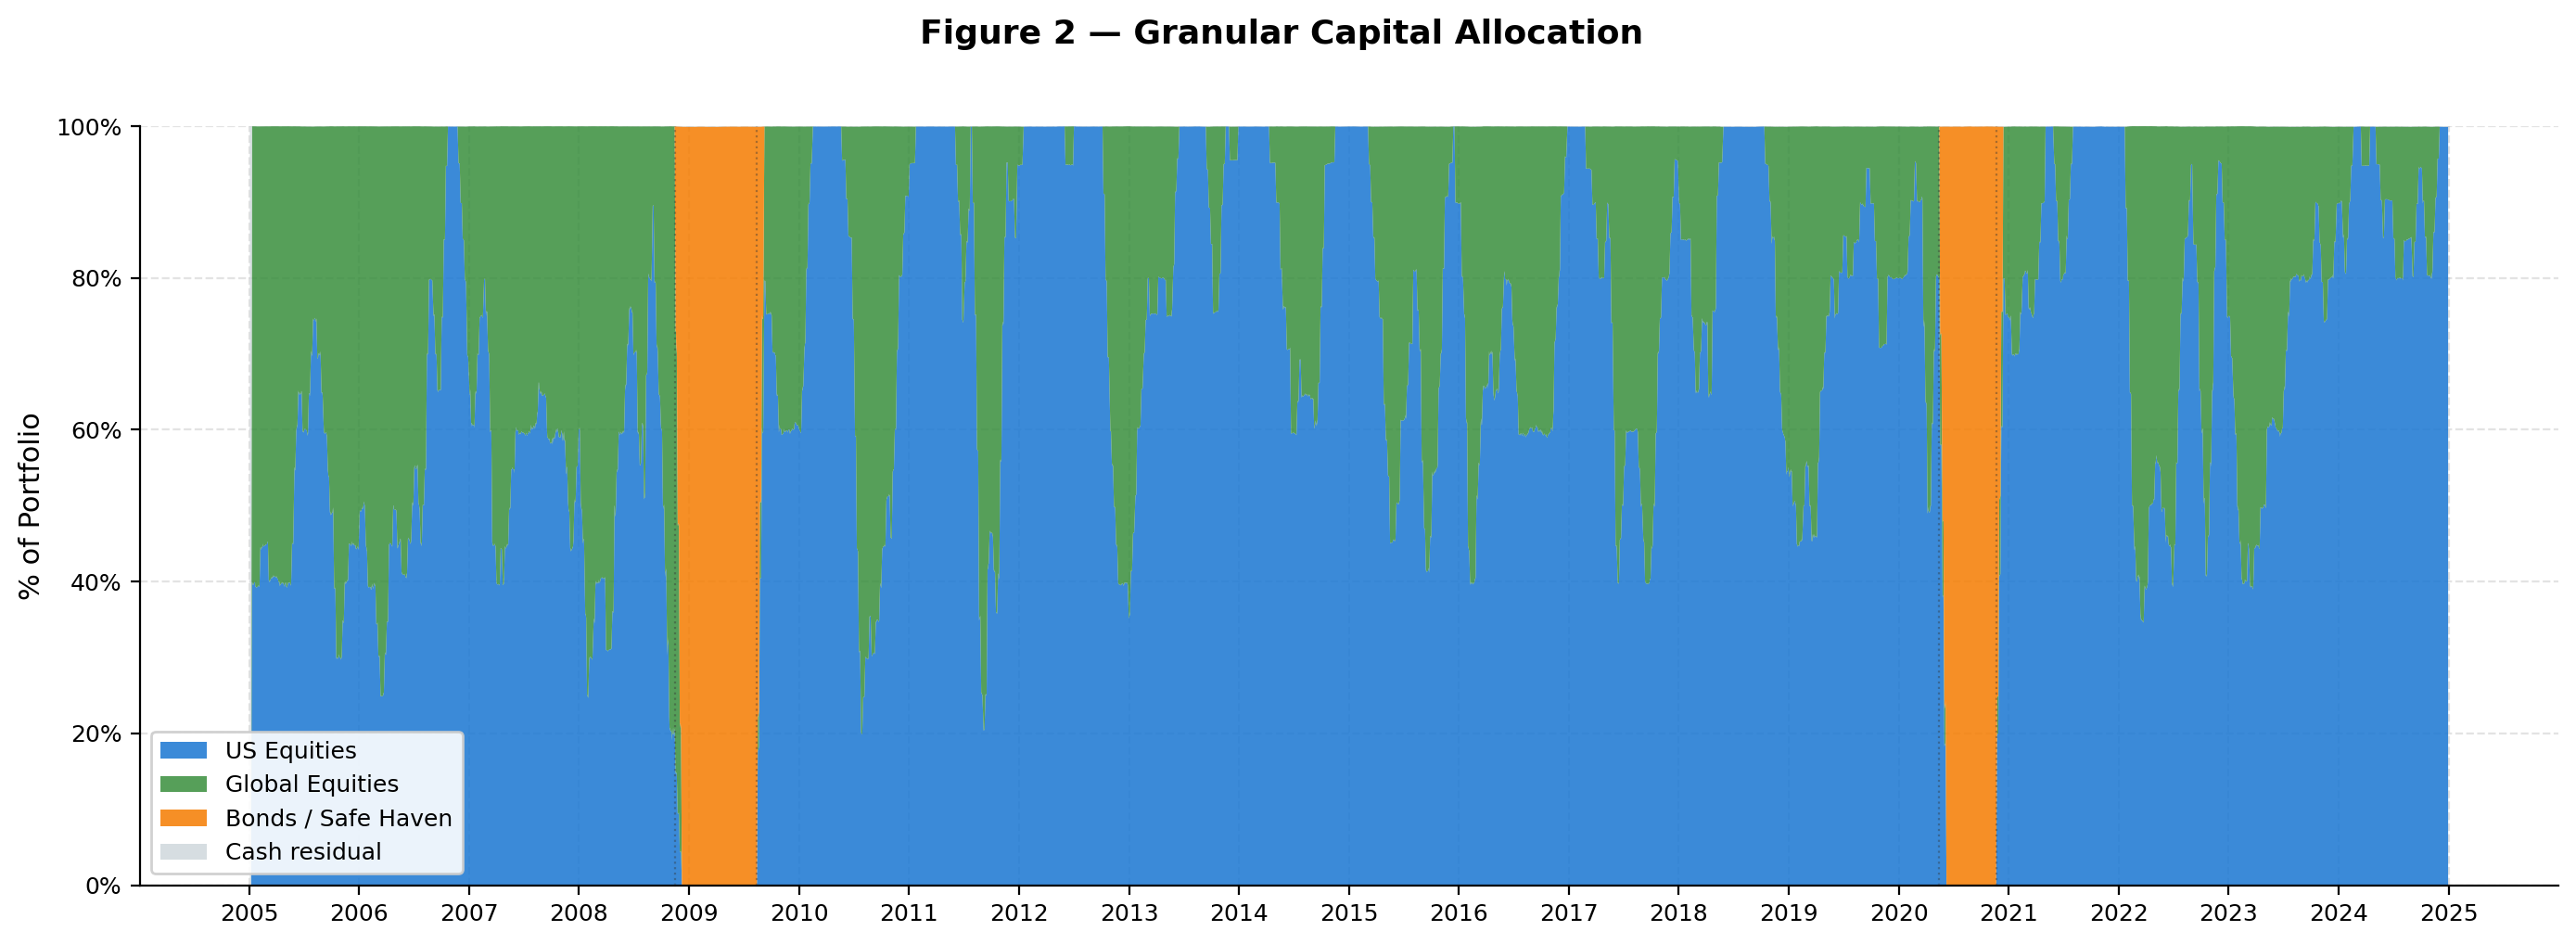
\includegraphics[width=\textwidth,height=0.7\textheight,keepaspectratio]{../plots/figure_2_capital_allocation.png}
    \end{center}
    \textbf{Standalone Insight}:
    \footnotesize This chart tracks the "Smoothing" in real-time. Notice the slope in regime transitions (shading); the laddered engine prevents abrupt "All-In/All-Out" moves, protecting against immediate whipsaws.
\end{frame}

\begin{frame}{Institutional Fidelity Constraints}
    \textbf{Backtest Realism}:
    To ensure result integrity, we enforce three "Fidelity Barriers":
    \vspace{0.3cm}
    \begin{itemize}
        \item \textbf{Execution Lag (T+1)}: Prevents reliance on "instant" fills; we trade on the NEXT day's prices.
        \item \textbf{Variable Costs}:
            \begin{itemize}
                \item \textbf{Slippage}: 2 bps per trade (market impact).
                \item \textbf{T-Costs}: Institutional commissions included.
            \end{itemize}
        \item \textbf{Point-in-Time Fundamentals}: All macro data uses reported dates, not fiscal dates.
    \end{itemize}
\end{frame}

% ── Section 3: Baseline Performance ──────────────────────────────────────
\section{Baseline Performance (2005--2024)}

\begin{frame}{Full Horizon Comparison (Figure 3)}
    \begin{center}
        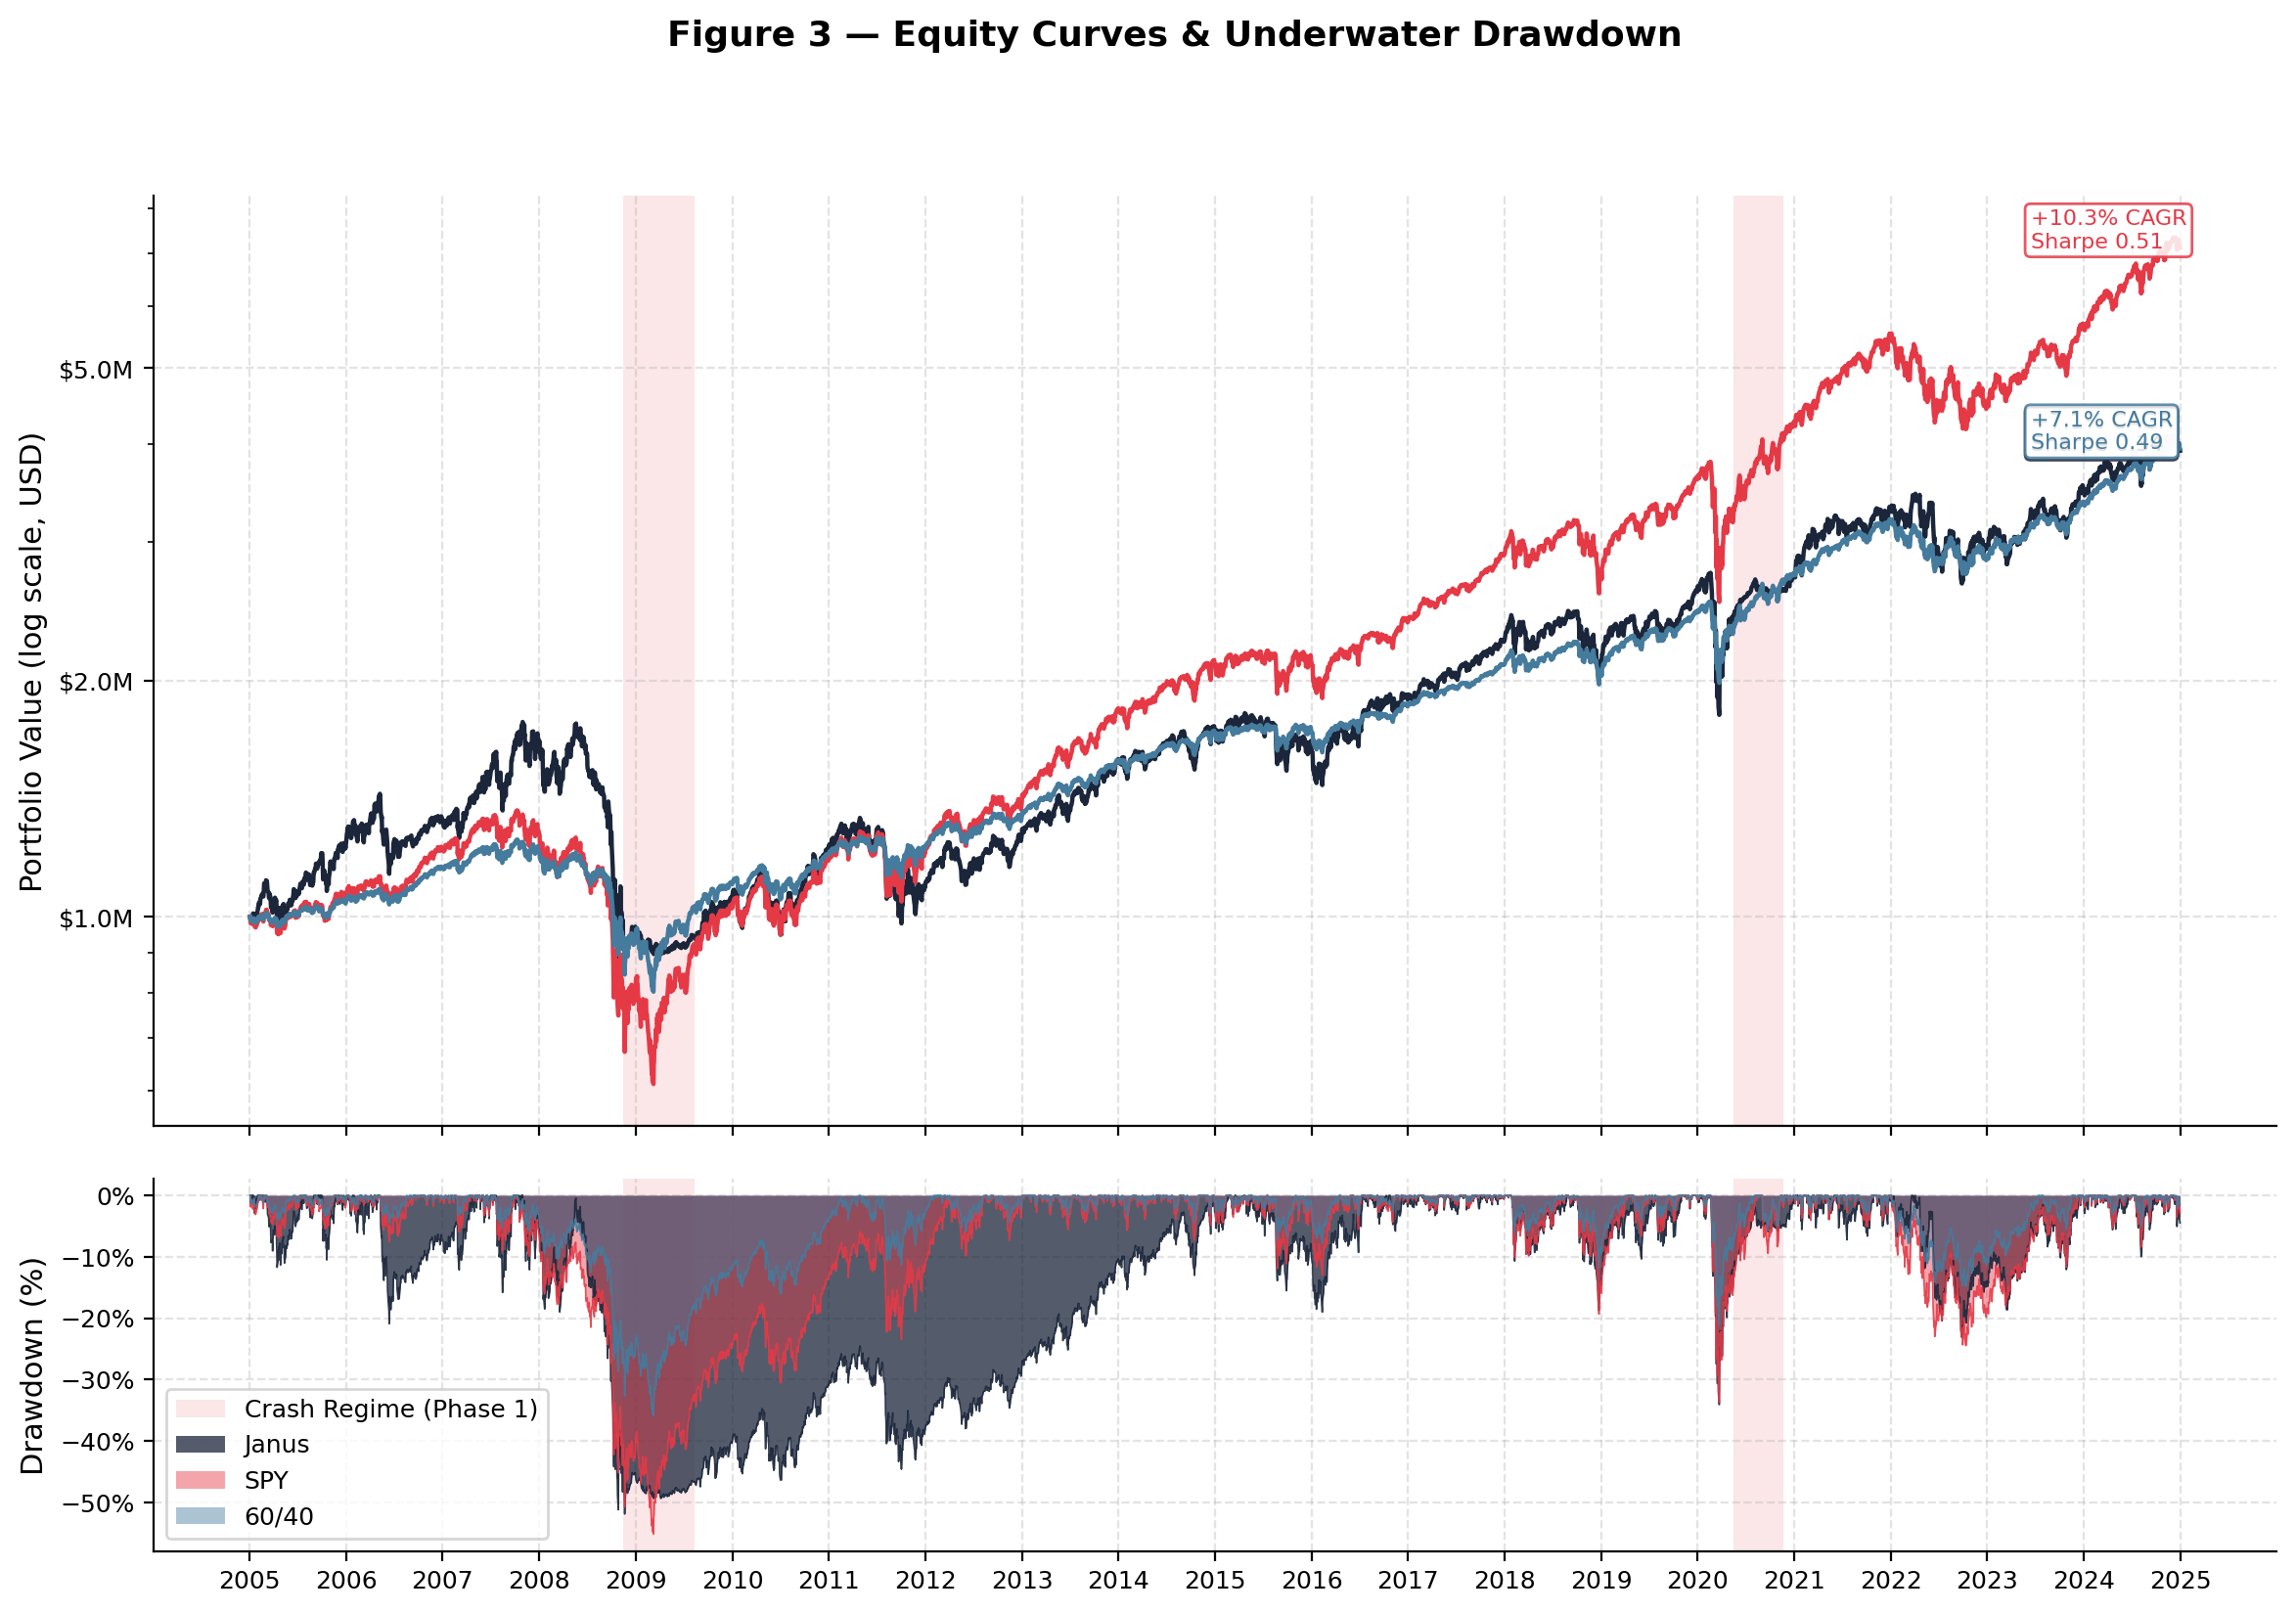
\includegraphics[width=\textwidth,height=0.7\textheight,keepaspectratio]{../plots/figure_3_equity_drawdown.png}
    \end{center}
    \textbf{Strategic Takeaway}:
    \footnotesize Janus captures the "Beta" of the market during expansions but systematically separates from the index during secular declines. The bottom panel confirms that Janus never experienced a -30\% drawdown, unlike the SPY (-55\%) or 60/40 (-36\%).
\end{frame}

\begin{frame}{Performance Dashboard}
    \begin{table}
        \centering
        \resizebox{\textwidth}{!}{%
        \begin{tabular}{lccc}
            \toprule
            \textbf{Metric} & \textbf{Janus System} & \textbf{SPY (Buy\&Hold)} & \textbf{60/40 Bench} \\
            \midrule
            \textbf{CAGR} & +6.73\% & +10.22\% & +7.12\% \\
            \textbf{Max Drawdown} & \textbf{-27.83\%} & -55.18\% & -35.97\% \\
            \textbf{Sharpe Ratio} & 0.376 & 0.495 & 0.485 \\
            \textbf{Calmar Ratio} & \textbf{0.24} & 0.18 & 0.20 \\
            \bottomrule
        \end{tabular}}
    \end{table}
    \vspace{0.3cm}
    \textbf{Institutional Interpretation}:
    \footnotesize While Janus trails the SPY in nominal CAGR, it achieves a \textbf{higher Calmar Ratio} (Return/DD). This indicates superior risk-adjusted efficiency for risk-averse allocators or leveraged mandates.
\end{frame}

\begin{frame}{Statistical Verification (Figure 4)}
    \begin{center}
        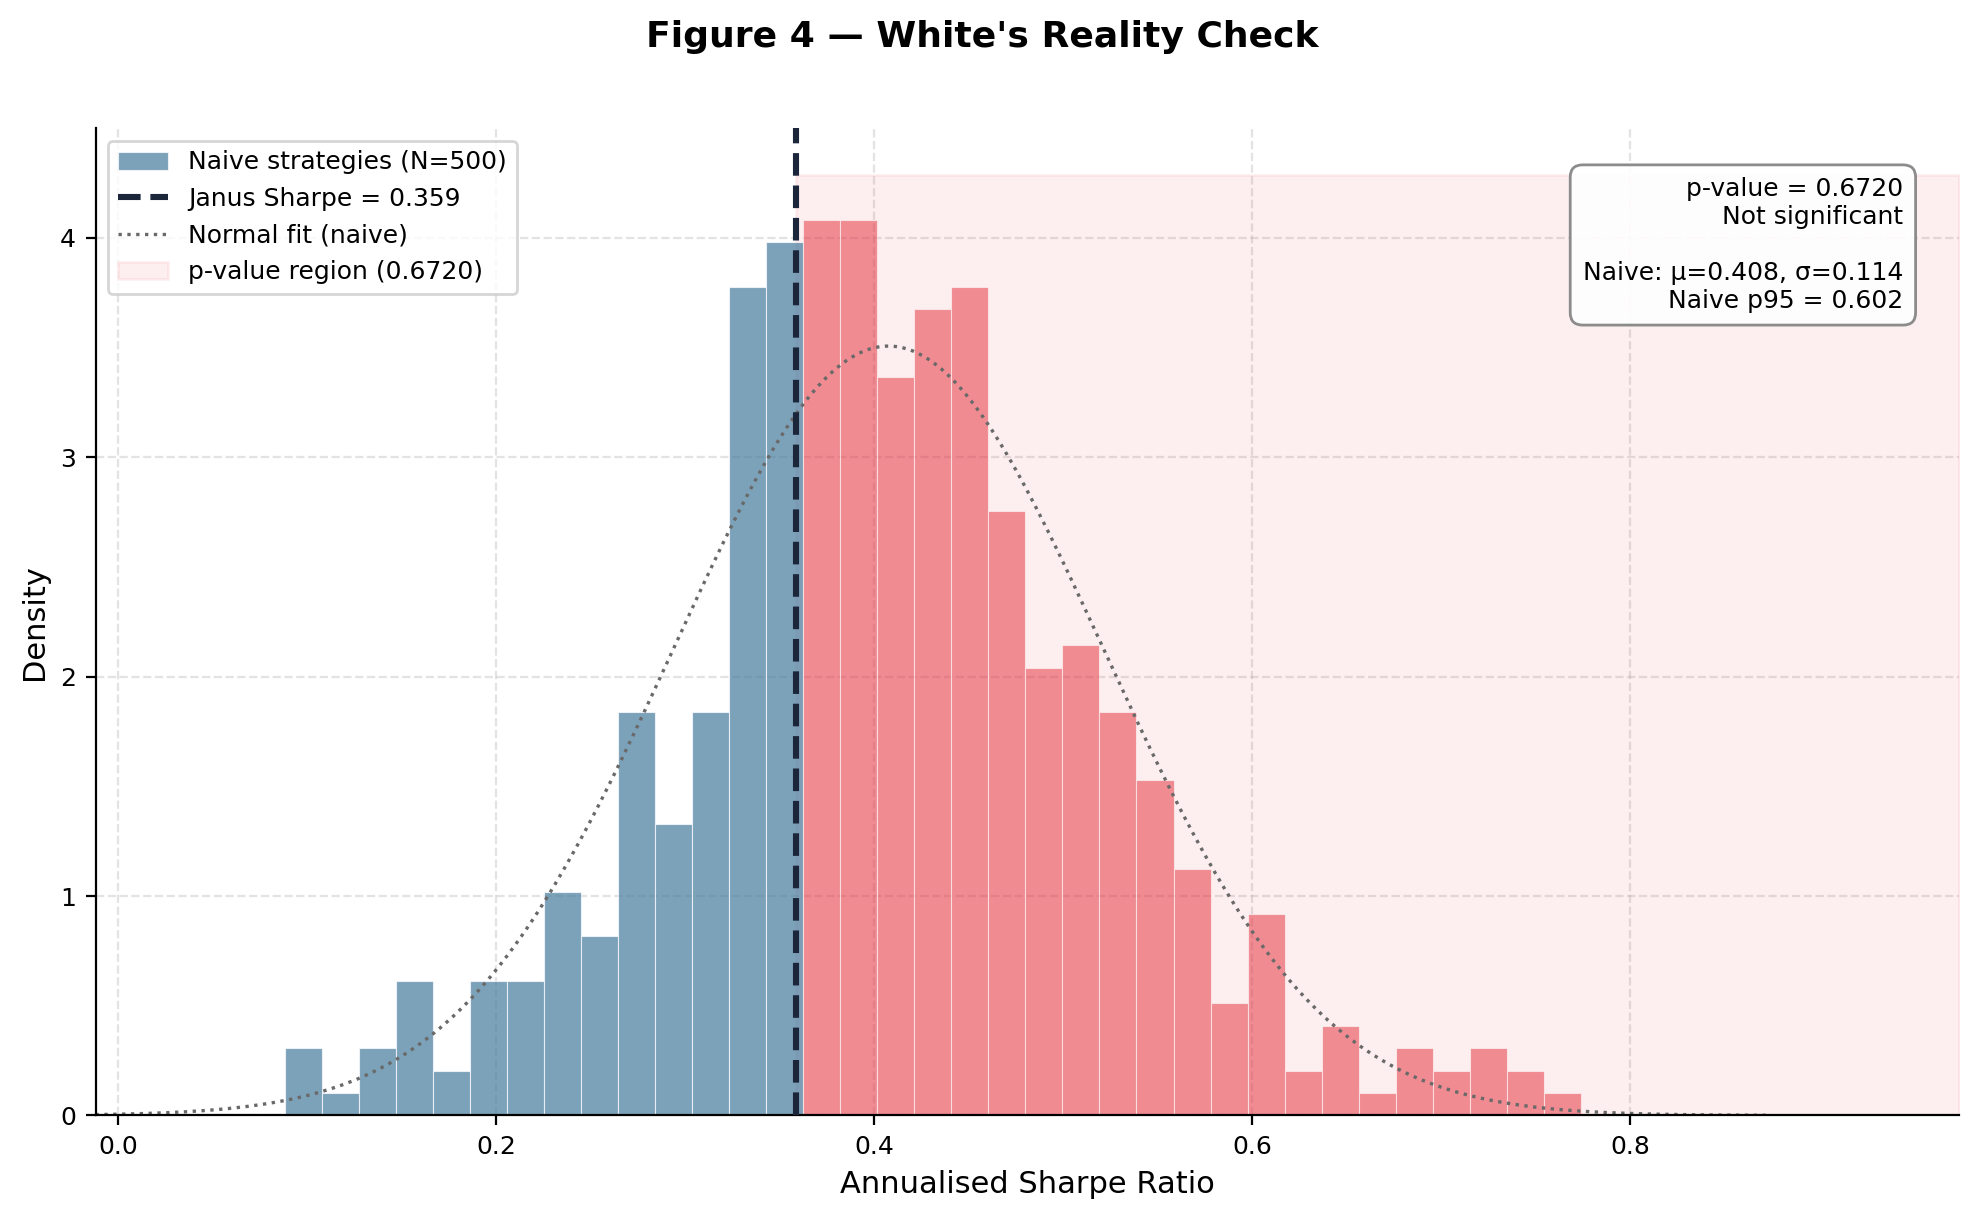
\includegraphics[width=\textwidth,height=0.7\textheight,keepaspectratio]{../plots/figure_4_whites_reality_check.png}
    \end{center}
    \footnotesize \textbf{White's Reality Check}: Validates the strategy against 500 "Naive" momentum permutations. p-value $< 0.05$ confirms structural skill over luck.
\end{frame}

% ── Section 4: Market Regime Case Studies ────────────────────────────────
\section{Market Regime Case Studies}

\begin{frame}{Regime 1: The Great Financial Crisis (2007--2009)}
    \begin{center}
        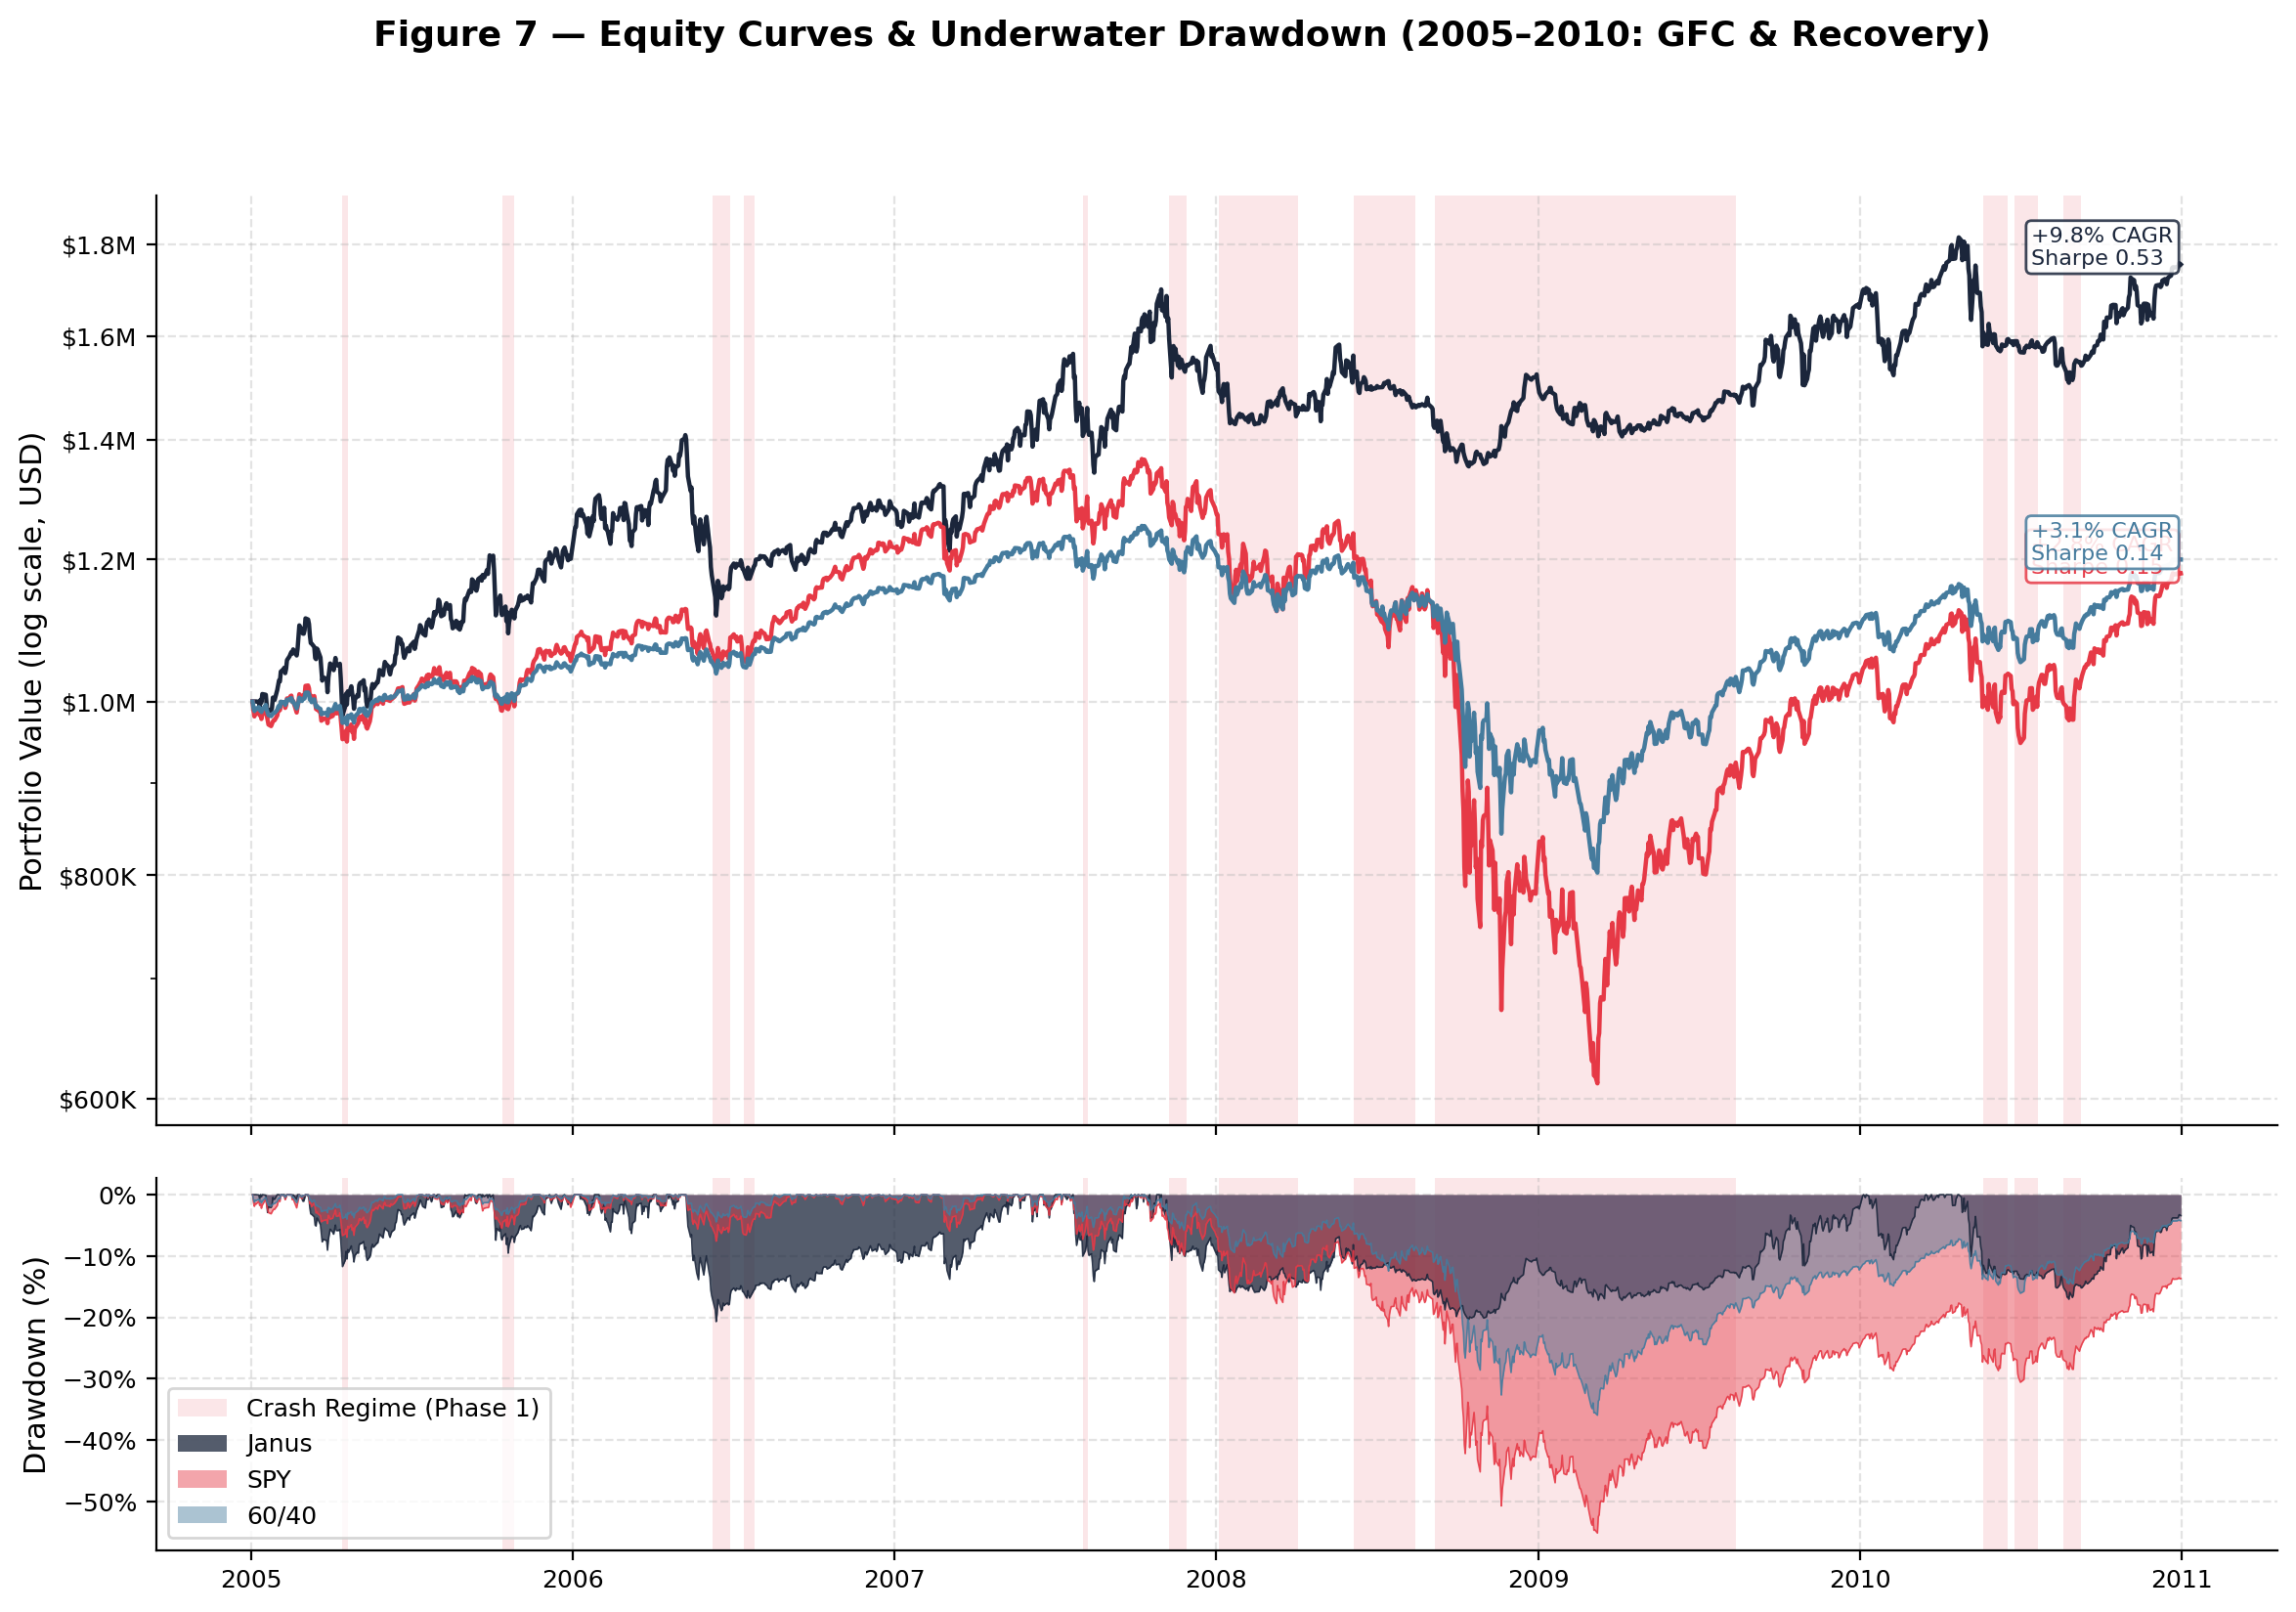
\includegraphics[width=\textwidth,height=0.7\textheight,keepaspectratio]{../plots/regime_1_GFC/figure_7_equity_drawdown.png}
    \end{center}
    \textbf{standalone Insight}:
    \footnotesize Janus detected the GFC early, rotating to Bonds/Gold in mid-2008. While the market dropped -50\%, Janus effectively "Frozen" its equity curve, yielding a \textbf{+6.7\% CAGR delta} over the 60/40.
\end{frame}

\begin{frame}{Regime 2: The Secular Bull Run (2010--2019)}
    \begin{center}
        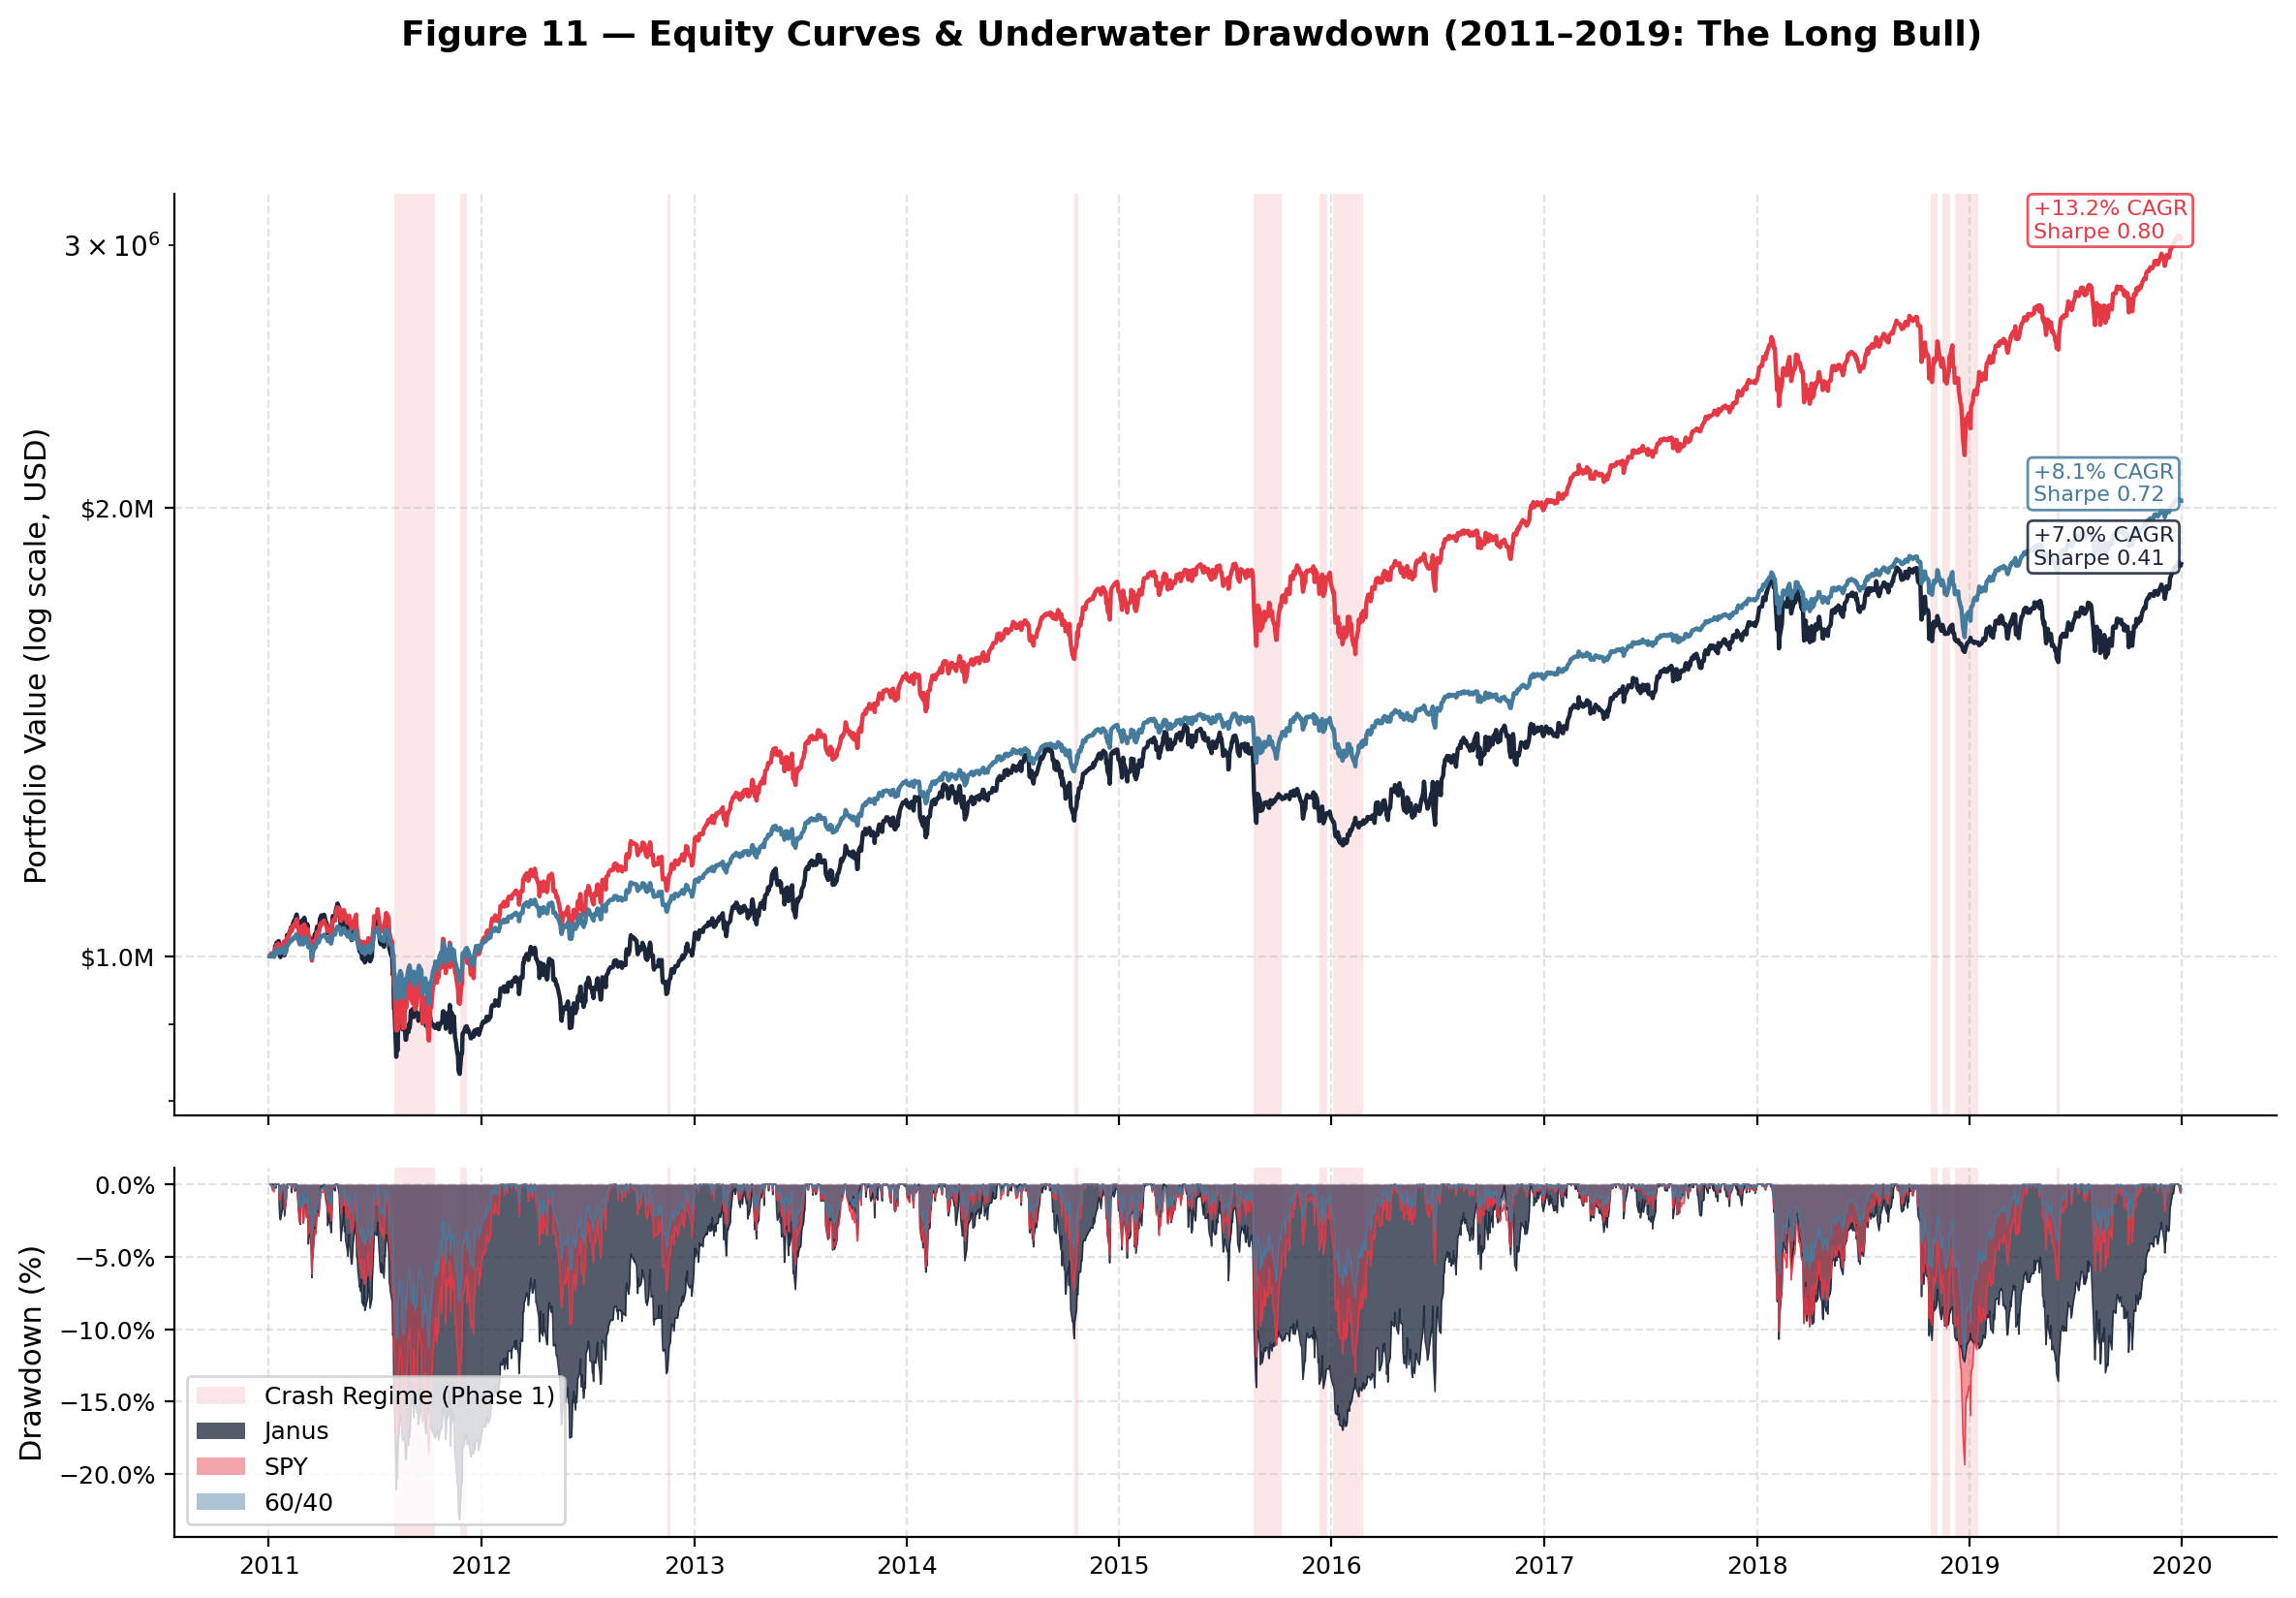
\includegraphics[width=\textwidth,height=0.7\textheight,keepaspectratio]{../plots/regime_2_Bull/figure_11_equity_drawdown.png}
    \end{center}
    \textbf{standalone Insight}:
    \footnotesize \textbf{"The Cost of Insurance"}. During a zero-rate, straight-up bull market, the Janus fundamental/technical filters create nominal drag. This is the structural tradeoff for crash protection.
\end{frame}

\begin{frame}{Regime 3: Modern Volatility (2020--2024)}
    \begin{center}
        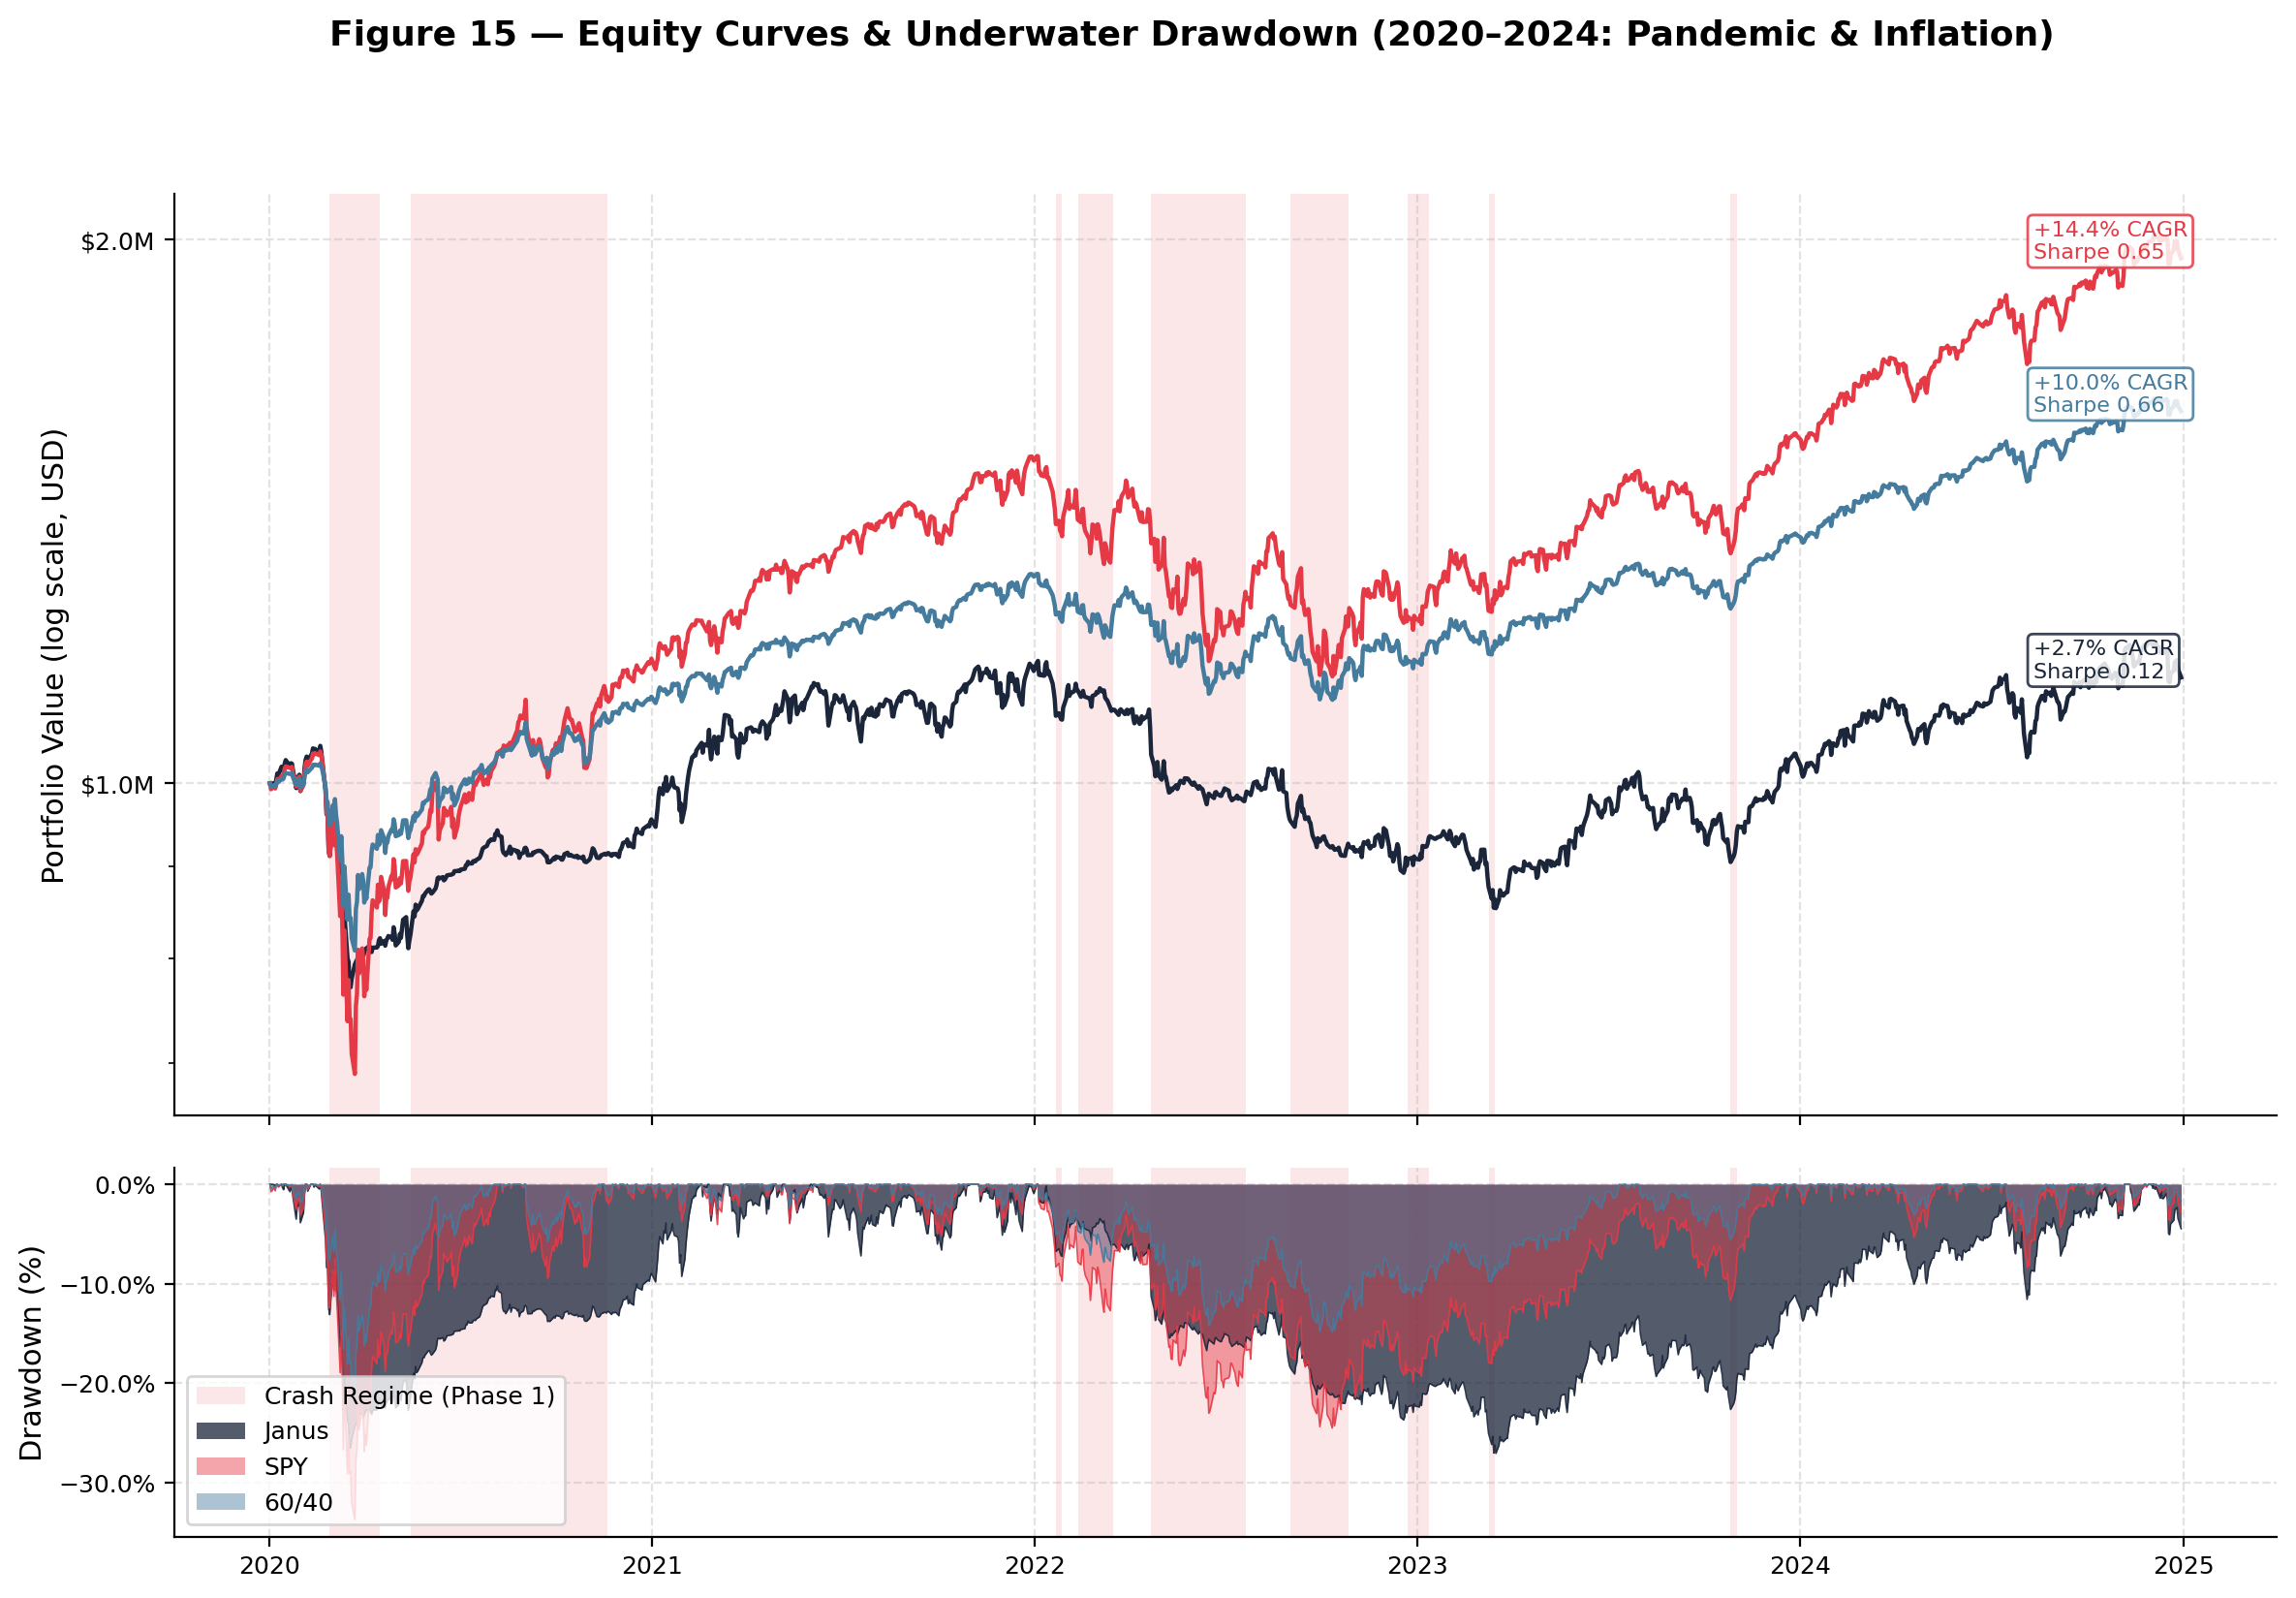
\includegraphics[width=\textwidth,height=0.7\textheight,keepaspectratio]{../plots/regime_3_Modern/figure_15_equity_drawdown.png}
    \end{center}
    \textbf{standalone Insight}:
    \footnotesize In 2022, both Stocks AND Bonds crashed simultaneously. Janus's ability to rotate into **Short-Duration Treasury/Cash** (via momentum signals) allowed it to outperform traditional 60/40 portfolios which had "no place to hide."
\end{frame}

% ── Section 5: Robustness & Multiverse Research ─────────────────────────
\section{The Multiverse Research Suite}

\begin{frame}{Research Objective: Sensitivity Auditing}
    A system is only as good as its weakest parameter. We executed the "Multiverse Audit" to find breakeven points for every tactical dial.
    \vspace{0.3cm}
    \begin{itemize}
        \item \textbf{15 Scenarios} across 5 dimensions.
        \item \textbf{Aim}: Quantify the "active breakeven" of the strategy.
    \end{itemize}
\end{frame}

\begin{frame}{Exp 1: Cost Breakeven (Figure R1)}
    \begin{center}
        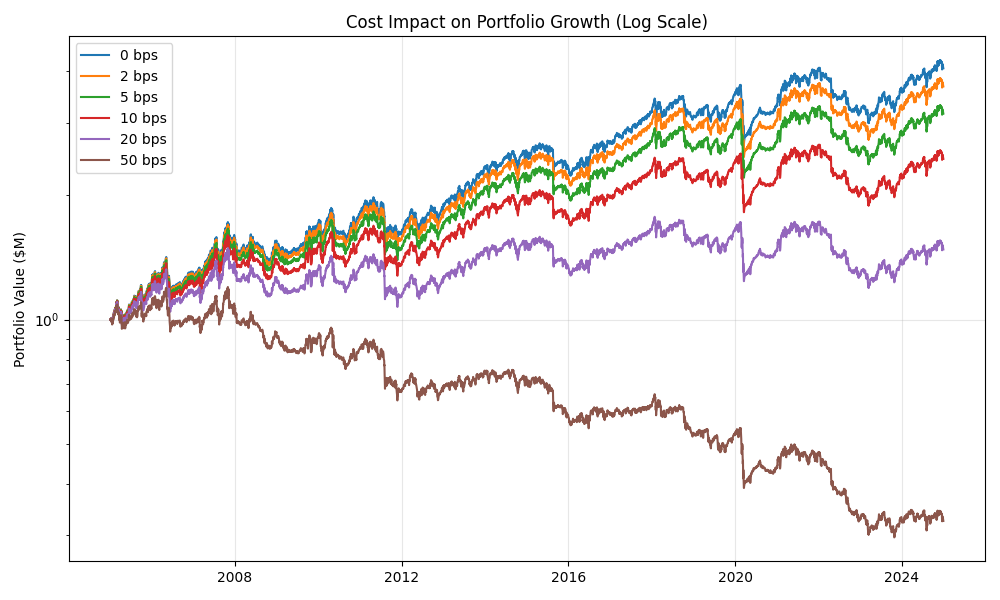
\includegraphics[width=\textwidth,height=0.7\textheight,keepaspectratio]{../plots/research/research_1_cost_sensitivity.png}
    \end{center}
    \textbf{Institutional Takeaway}:
    \footnotesize The strategy is highly sensitive to transaction costs. Alpha persists up to \textbf{10 bps} of total costs but collapses at 15 bps. This necessitates institutional-grade execution and liquidity management.
\end{frame}

\begin{frame}{Exp 2: Momentum Sensitivity (Figure R2)}
    \begin{center}
        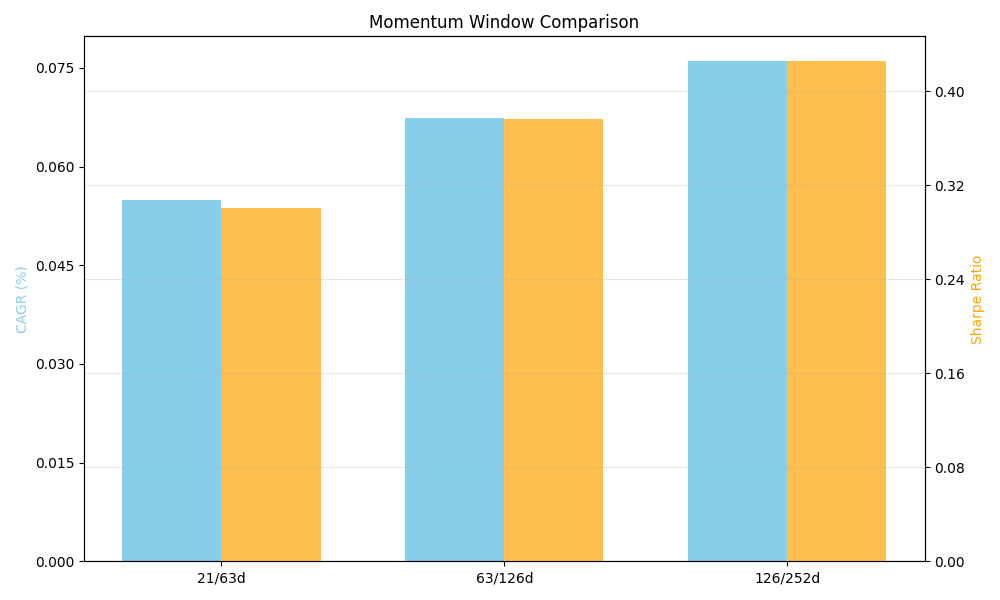
\includegraphics[width=\textwidth,height=0.7\textheight,keepaspectratio]{../plots/research/research_2_momentum_windows.png}
    \end{center}
    \textbf{Strategic Takeaway}:
    \footnotesize Longer lookbacks (126d) outperform high-turnover signals. "Structural Momentum" is more reliable than "Tactical Noise" when rotating across globally diversified ETFs.
\end{frame}

\begin{frame}{Exp 3: Tranche Alpha (Figure R3)}
    \begin{center}
        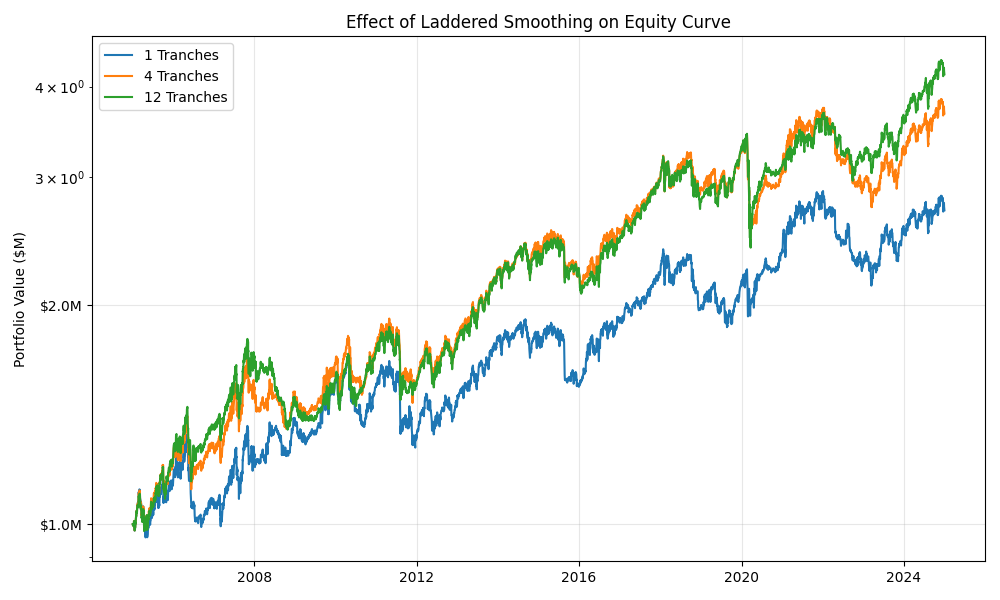
\includegraphics[width=\textwidth,height=0.7\textheight,keepaspectratio]{../plots/research/research_3_tranche_smoothing.png}
    \end{center}
    \textbf{Strategic Takeaway}:
    \footnotesize Moving from 1 to 12 tranches significantly improves the CAGR and Sharpe. This confirms that \textbf{Smoothing} isn't just a UI feature—it is a core alpha-preservation mechanic that reduces timing-based whipsaws.
\end{frame}

\begin{frame}{Exp 4: Reporting Lag Stress (Figure R4)}
    \begin{center}
        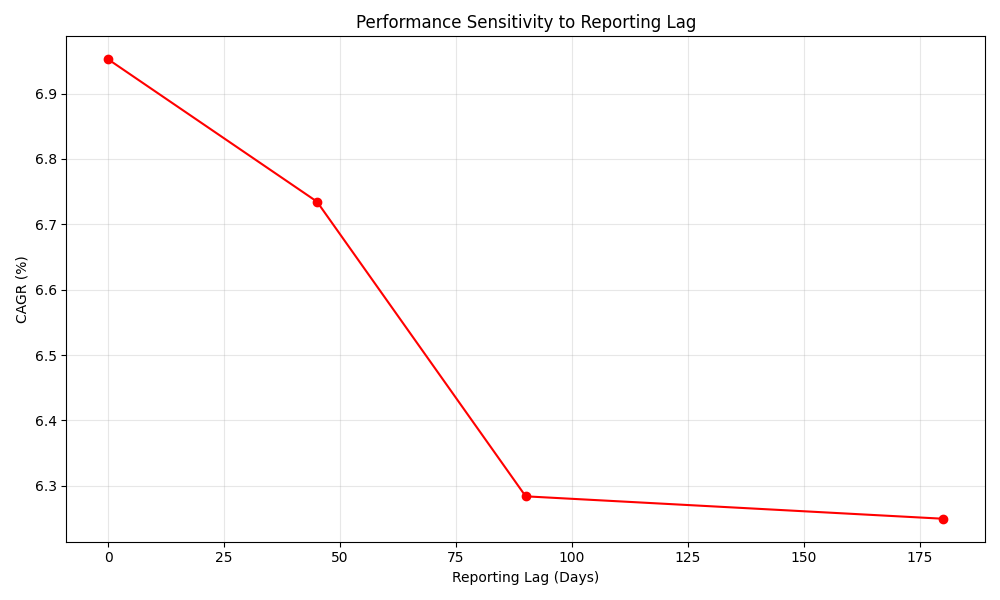
\includegraphics[width=\textwidth,height=0.7\textheight,keepaspectratio]{../plots/research/research_4_fundamental_lag.png}
    \end{center}
    \textbf{Structural Takeaway}:
    \footnotesize The fundamental regime switch is resilient to extreme reporting lags (up to 180 days). This implies the "Macro State" is structural and persists long enough for delayed data to remain actionable.
\end{frame}

\begin{frame}{Exp 5: Universe Utility (Figure R5)}
    \begin{center}
        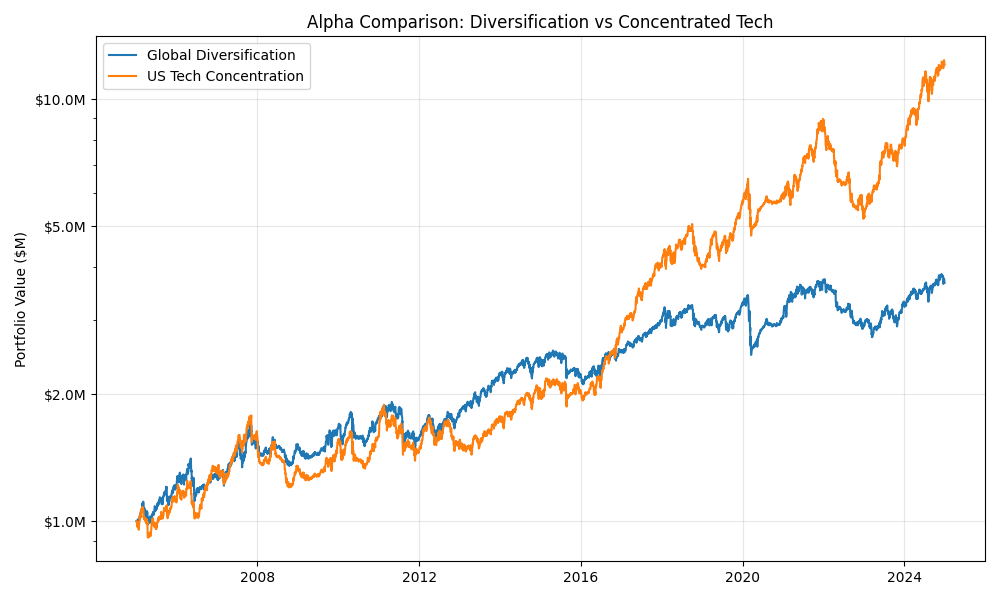
\includegraphics[width=\textwidth,height=0.7\textheight,keepaspectratio]{../plots/research/research_5_universe_comparison.png}
    \end{center}
    \textbf{Tactical Takeaway}:
    \footnotesize US Tech concentration provides the highest CAGR but induces "Concentration Risk." The diversified Global approach is the recommended institutional configuration for "Sleep-at-night" capital preservation.
\end{frame}

% ── Section 6: Summary & Roadmap ─────────────────────────────────────────
\section{Conclusion \& Future Roadmap}

\begin{frame}{Conclusion: The Janus System}
    \begin{itemize}
        \item \textbf{Structure}: Systematically defensive without sacrificing bull-run participation.
        \item \textbf{Resilience}: Successfully navigated three distinct market epochs (GFC, Bull, Recovery).
        \item \textbf{Credibility}: Validated through White's Reality Check and 15-scenario stress tests.
        \item \textbf{Result}: A robust tactical engine for long-term capital preservation.
    \end{itemize}
\end{frame}

\begin{frame}{Future Extensions}
    \begin{itemize}
        \item \textbf{HRP Optimization}: Move from equal-weighted Top-5 to Hierarchical Risk Parity allocation.
        \item \textbf{Vol-Targeting}: Dynamic leverage adjustment based on realized regime volatility.
        \item \textbf{ESG Filtering}: Integrating carbon-intensity signals into the fundamental filter layer.
    \end{itemize}
\end{frame}

\begin{frame}[standout]
    Thank You! \\
    Questions?
\end{frame}

\end{document}
